\chapter{损伤的修复}

\chapterabstract{本章主要介绍机体组织损伤后的修复过程,要求掌握修复、再生、纤维性修复、肉芽组织的概念,不同类型细胞的再生能力,肉芽组织的构成及其在修复过程中的作用,熟悉常见组织的再生过程,瘢痕组织的形态及对机体的影响,创伤愈合的基本过程和皮肤的创伤愈合,了解细胞再生的影响因素,骨折愈合过程和影响创伤愈合的因素。}
\begin{framed}
	{案例2-1}

	{【病例摘要】}

	患者,男,65岁,因意识不清,突发倒地入院。CT检查示右侧基底节出血灶,外科行血肿清除术后,生命体征平稳,但患者仍无自主意识,长期卧床。术后20天,患者左侧肩胛部见一压疮灶,直径约4
	cm,深部组织坏死明显,清创术后数日,见压疮灶内有红色颗粒状组织覆盖。

	{【问题】}

	(1)该压疮灶内红色颗粒状组织是什么?由哪些成分构成?

	(2)该红色颗粒状组织有何功能?
\end{framed}
机体对损伤所造成的缺损进行修补恢复的过程,称为修复(repair)。修复过程可包括两种不同的形式:由损伤周围邻近的同种细胞来修复,称为再生(regeneration);由纤维结缔组织来修复,最后局部纤维化,形成瘢痕,称为纤维性修复。

\section{再生}

\subsection{再生的类型}

\paragraph{生理性再生}
生理过程中,许多组织细胞不断衰老、死亡,同时又由同种细胞通过分裂增生补充,这种再生称为生理性再生。例如皮肤表层角化细胞经常脱落,表皮基底层细胞不断增生分化,予以补充,胃黏膜上皮三天左右更新一次,血细胞也在不断更新等,皆属生理性再生。

\paragraph{病理性再生}
在病理状态下,组织细胞坏死或缺损后,通过周围同种细胞增生来恢复原有的结构和功能,称为病理性再生。如皮肤表皮损伤后,基底层以上各层细胞坏死,由基底层细胞增生、分化,恢复表皮的结构和功能。

\subsection{不同类型细胞的再生能力}

按再生能力不同,将人体组织细胞分为三类。

\paragraph{不稳定细胞(Labile cells)}
这类细胞再生能力强,在生理状态下经常进行周期活动,不断分裂增生,以补充衰老死亡的细胞,在病理状态下也具有强大的再生能力。例如全身的上皮细胞、淋巴造血细胞。上皮细胞包括皮肤表皮、胃肠道和呼吸道的黏膜上皮、泌尿道的移行上皮以及腺体的导管上皮等。

\paragraph{稳定细胞(stable cells)}
这类细胞在生理状态下增生现象不明显,处于细胞增殖周期的静止期(G{0}
期),但具有潜在的再生能力,在损伤的刺激下,则进入DNA合成前期(G{1}
期),表现出较强的再生能力。属于这类细胞的有各种腺体及腺样器官的实质细胞,如肝、胰、内分泌腺、汗腺、皮脂腺及肾小管的上皮细胞等;还包括间叶细胞及其衍生的各种细胞,例如成纤维细胞、骨、软骨、脂肪、平滑肌细胞等。

\paragraph{永久性细胞(permanent cells)}
这类细胞在生理状态下较为恒定,基本上无再生能力,故不能分裂增生,一旦遭受损伤则成为永久性缺失。属于这类的细胞有神经细胞、心肌细胞及骨骼肌细胞。心肌细胞和骨骼肌细胞虽有微弱的再生能力,但因速度极慢,以至损伤处被快速增生的纤维结缔组织替代,通过瘢痕修复。

\subsection{常见组织的再生过程}

\paragraph{上皮组织的再生}
(1)被覆上皮再生:皮肤的复层鳞状上皮受损伤时,创缘或基底部残存的基底细胞则分裂、增生,向缺损中心移动。初起为单层,完全覆盖缺损后,细胞开始分化,形成多层,以后角化。黏膜上皮也以同样的方式再生,新生的黏膜上皮细胞初起为立方形,以后增高变为柱状。

(2)腺上皮再生:腺体受损伤后,若基底膜未被破坏,残存的腺上皮分裂增生,可恢复原有的结构和功能。若腺体(包括基底膜)完全破坏,则难以再生。肝细胞有活跃的再生能力,但如肝内网状支架塌陷,再生的肝细胞则形成结构紊乱的肝细胞结节。

\paragraph{血管的再生}
毛细血管多以出芽方式再生。原有毛细血管内皮细胞肥大、分裂增生,形成向血管外突起的幼芽。开始幼芽为实心的细胞条索,在血流冲击下形成管腔,并有血液通过,进而互相吻合构成毛细血管网(图\ref{fig2-1})。为适应功能需要,毛细血管不断改建,部分管腔关闭消失,部分管壁增厚,成为小动脉、小静脉,其平滑肌等成分可由血管外未分化的间叶细胞分化而来。

大血管离断后需手术吻合,吻合处两侧的内皮细胞分裂增生,互相连接,恢复原来的内膜结构。离断处的肌层难以再生,由结缔组织连接,通过瘢痕修复。

\paragraph{纤维组织再生}
纤维组织普遍分布于机体各部位,再生能力很强,是病理性再生中最常见的现象。在损伤的刺激下,局部静止状态的纤维细胞,或未分化的间叶细胞分化形成幼稚的纤维母细胞。幼稚的纤维母细胞胞体大、胞浆丰富略嗜碱性,两端常有突起。电镜下胞浆内有丰富的粗面内质网和高尔基器,提示其合成蛋白的功能活跃。当纤维母细胞停止分裂后,开始合成并分泌原胶原蛋白,在细胞周围形成胶原纤维。随着细胞的成熟,周围胶原纤维逐渐增多,于是胞体大、有突起的纤维母细胞则变成长梭形的半静止状态的纤维细胞(图\ref{fig2-2})。
\begin{figure}[!h]
	\begin{center}
		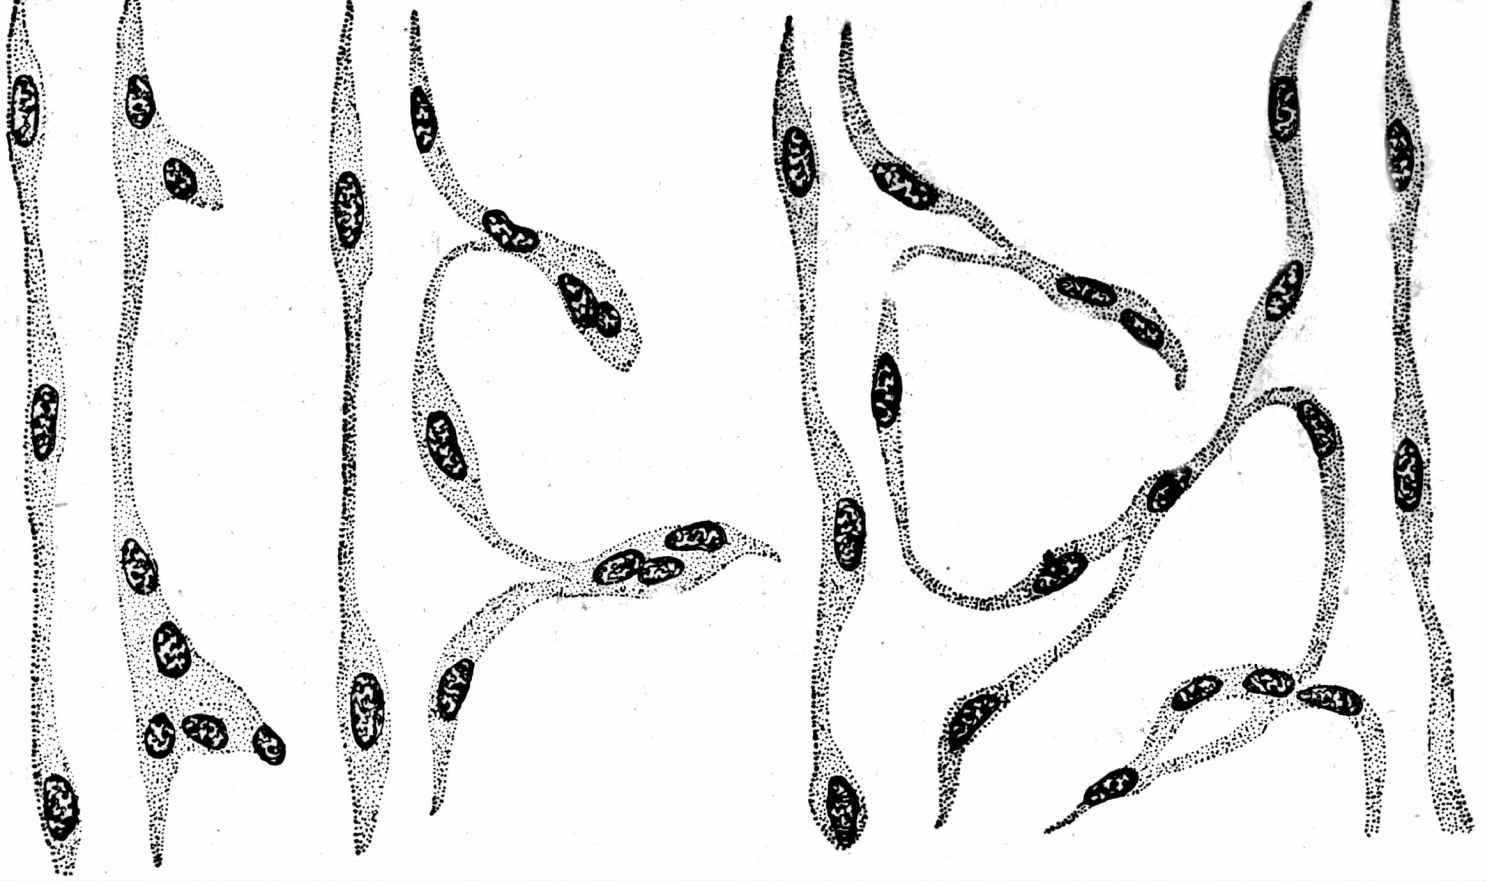
\includegraphics{./images/Image00024.jpg}
	\end{center}
	\captionsetup{justification=centering}
	\caption{毛细血管再生模式图 \\ {\small 毛细血管内皮细胞增生;增生的内皮细胞形成条索,并出现管腔;新生的毛细血管相互连接、沟通}}
	\label{fig2-1}
\end{figure}
%\FloatBarrier


\begin{figure}[!h]
	\begin{center}
		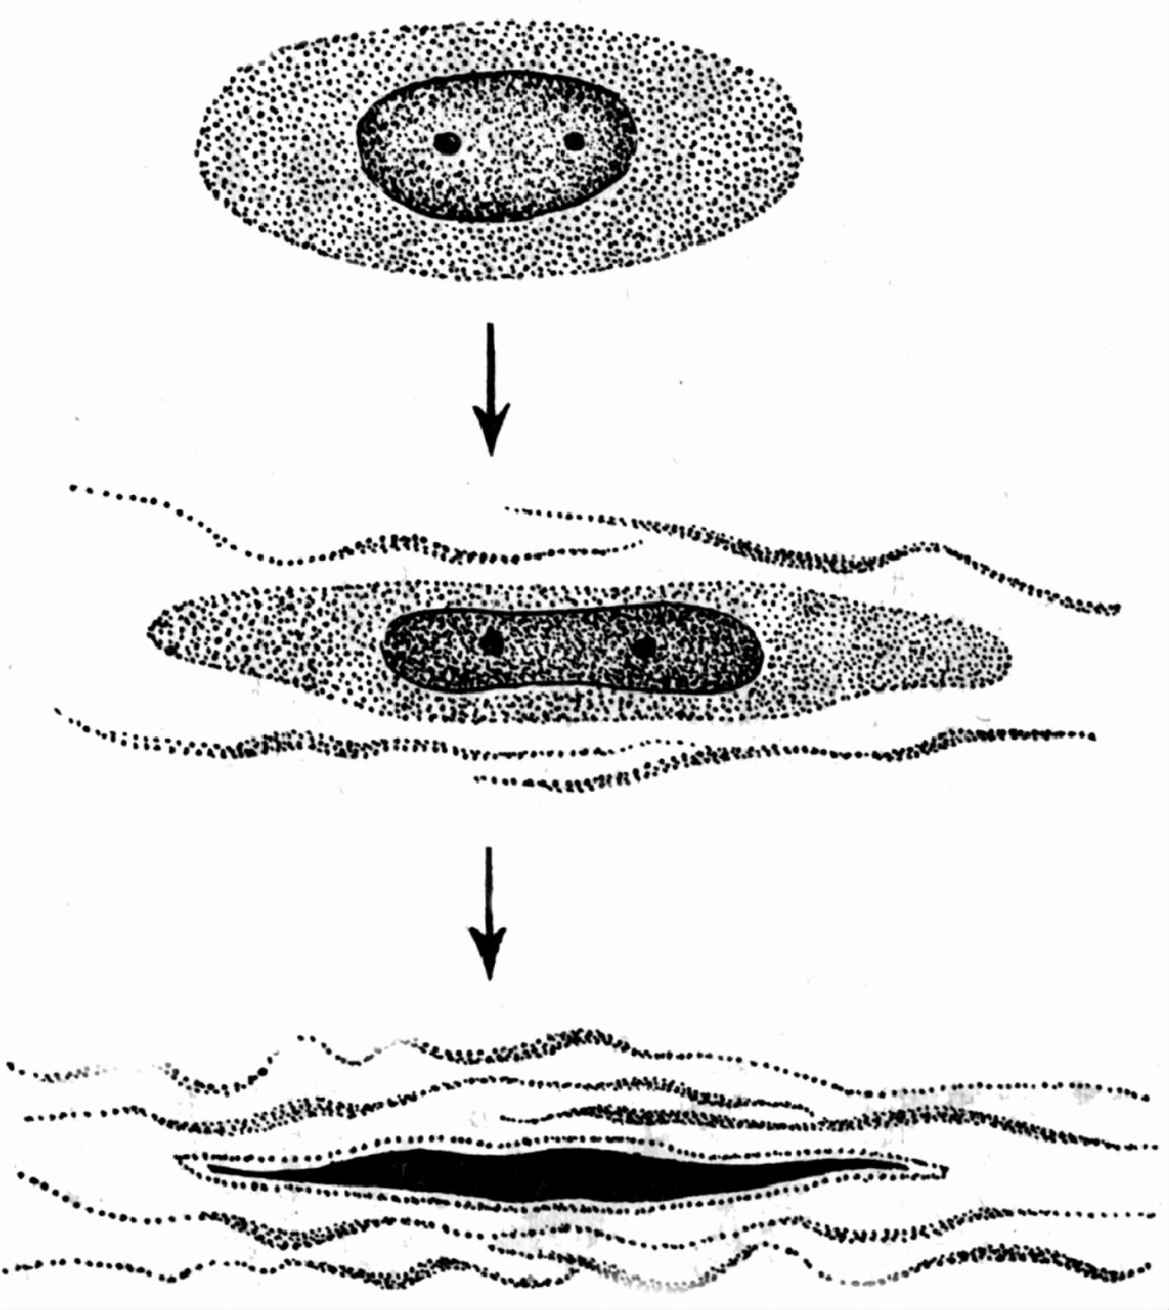
\includegraphics{./images/Image00025.jpg}
	\end{center}
	\captionsetup{justification=centering}
	\caption{纤维母细胞产生胶原纤维并转变为纤维细胞的模式图}
	\label{fig2-2}
\end{figure}
%\FloatBarrier

\paragraph{神经组织的再生}
脑和脊髓内的神经细胞破坏后不能再生,由再生能力较强的胶质细胞形成胶质纤维填补,形成胶质瘢痕。但神经纤维断离后,如果与其相连的神经细胞仍然存活,则可再生。首先断处远侧端的神经髓鞘及轴突崩解吸收,断处近侧一小段神经纤维亦发生同样变化。然后两端的神经膜细胞增生,将断端连接,并产生髓磷脂将轴突包绕,形成髓鞘。近端新生的轴突伸向远端髓鞘内,最终达到该神经末稍,可以完全恢复其功能。由于神经轴突生长缓慢(每天延长1~2
mm),再生过程常需数月以上才能完成。如果近端再生的神经轴突未能向远端髓鞘内伸展,只在断裂处长出很多细支,与周围增生的纤维组织缠绕在一起,可形成瘤状物,即创伤性神经瘤(traumatic
neuroma),可引起顽固性疼痛。为防止上述情况发生,临床上常施行神经吻合术或对截肢神经断端作适当处理。

\section{纤维性修复}

纤维性修复开始于肉芽组织增生,填补组织缺损,以后肉芽组织经过纤维化的过程,转化为胶原纤维为主的瘢痕组织,这种修复便告完成。

\subsection{肉芽组织}

肉芽组织(granulation
tissue)由新生的毛细血管、增生的纤维母细胞及多少不等的炎细胞组成,在创伤表面常呈鲜红色,颗粒状,柔软湿润,似新鲜肉芽(图\ref{fig2-3}),故此得名。组织损伤后24小时内,血管内皮细胞及纤维母细胞开始增生,新生的毛细血管管壁的基底膜和胶原纤维尚不完整,故血管通透性大,富有蛋白的液体甚至红细胞漏出到血管外间隙,使肉芽组织呈水肿样外观。新生的毛细血管常呈平行排列,与创面垂直生长,近伤口表面处互相吻合,形成弓状突起。与此同时,局部组织的纤维母细胞受刺激,分裂增生,并产生胶原纤维(图\ref{fig2-4})。毛细血管与血管之间增生的纤维母细胞一起构成小团块,均匀分布,突起于创面,呈颗粒状。肉芽组织中有些细胞外形似纤维母细胞,除能产生胶原纤维外,胞浆中还含有丰富的肌动蛋白和肌凝蛋白,电镜下胞浆内具有丰富的肌微丝,具有类似平滑肌的收缩能力,这种变异的细胞被称为肌纤维母细胞,在创伤收缩中起重要作用。肌纤维母细胞的起源不明,可能来自未分化的间叶细胞,也可能是一种特殊分化的纤维母细胞。炎细胞中以巨噬细胞为主,也可有中性粒细胞及淋巴细胞。巨噬细胞和中性粒细胞具有吞噬细菌和组织碎片的作用,这些细胞坏死后释放的蛋白水解酶能分解坏死组织及纤维蛋白。

\begin{figure}[!h]
	\begin{center}
		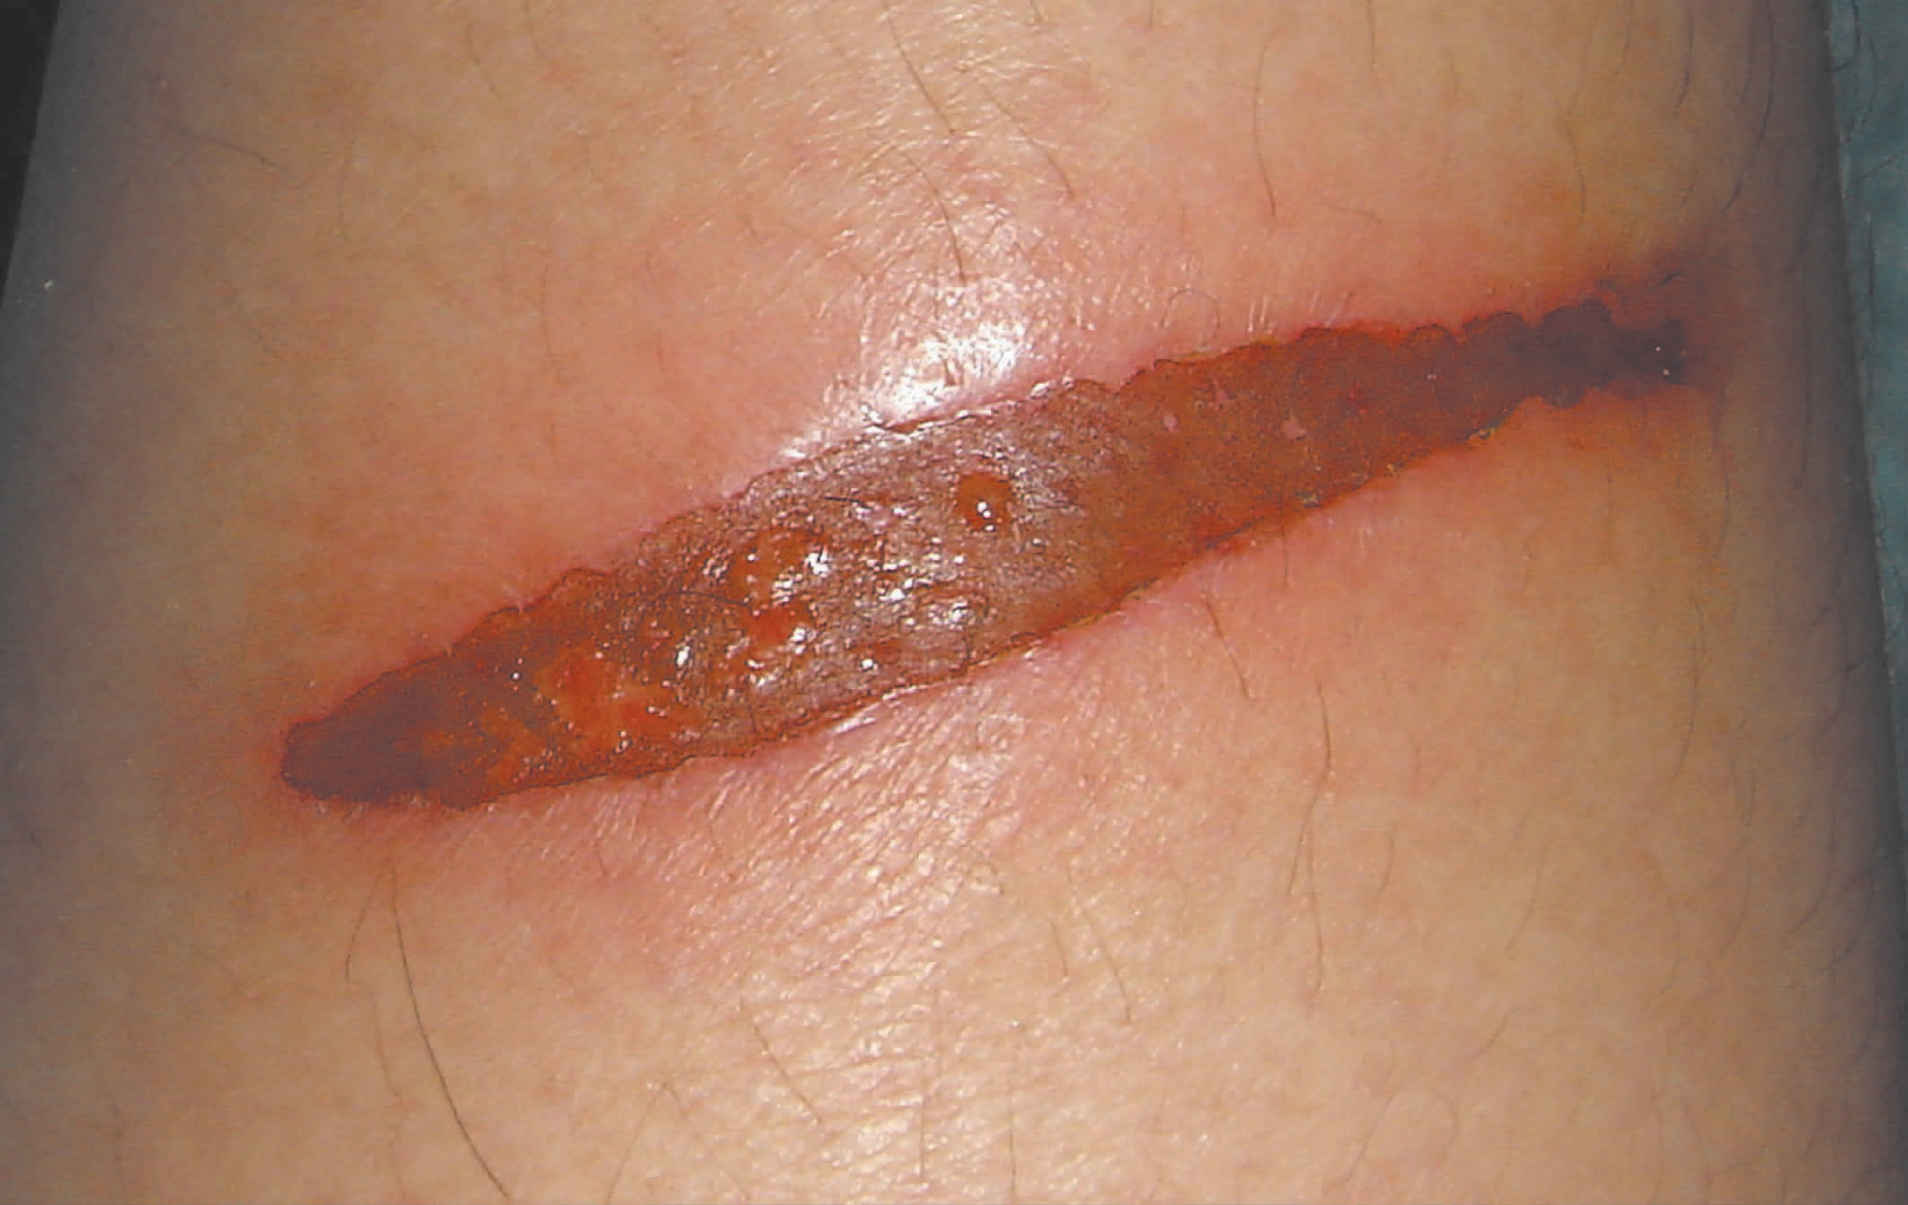
\includegraphics{./images/Image00026.jpg}
	\end{center}
	\captionsetup{justification=centering}
	\caption{创口表面颗粒状肉芽组织}
	\label{fig2-3}
\end{figure}


\begin{figure}[!h]
	\begin{center}
		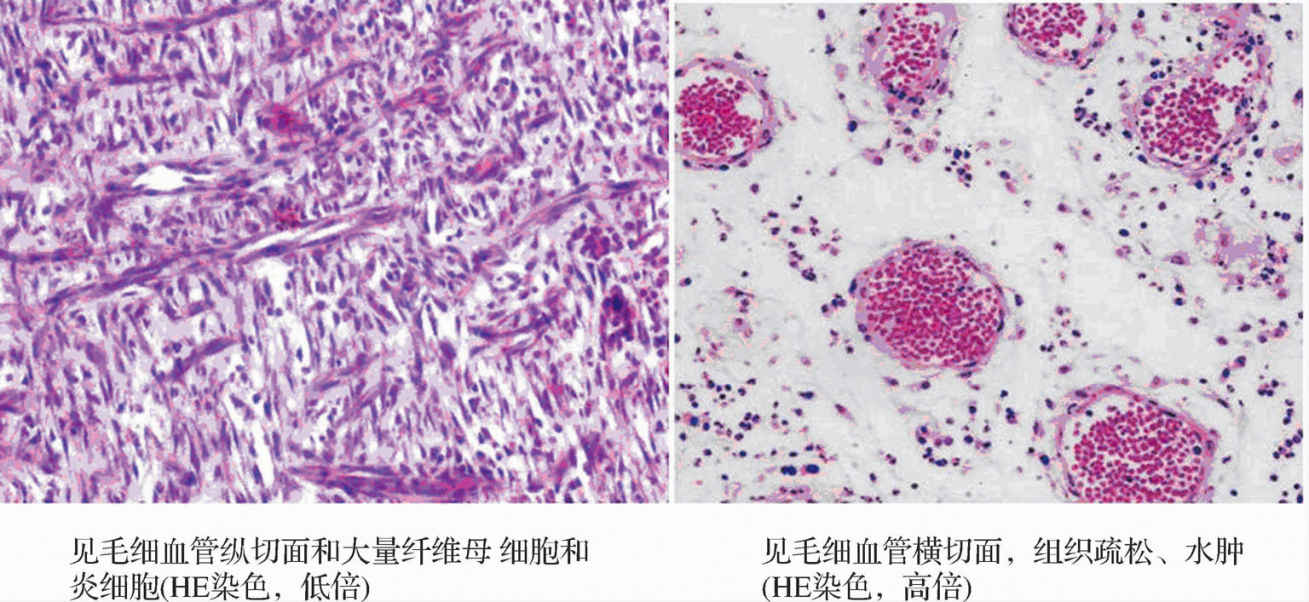
\includegraphics{./images/Image00027.jpg}
	\end{center}
	\captionsetup{justification=centering}
	\caption{肉芽组织镜下观}
	\label{fig2-4}
\end{figure}

肉芽组织在修复过程中有抗感染及保护创面,机化血凝块、坏死组织及其他异物,填补伤口或其他组织缺损等作用。

\subsection{瘢痕组织}

肉芽组织形成的初期呈鲜红色、颗粒状,如嫩芽,以后细胞间水分逐渐减少,纤维母细胞合成胶原纤维,并逐渐转变为纤维细胞。随着细胞外胶原纤维增多,多数毛细血管逐渐关闭、退化、消失,少数改建为小动脉、小静脉。肉芽组织中的炎细胞也先后消失。经过上述纤维化过程,肉芽组织转变为血管稀少,主要由胶原纤维组成的瘢痕组织(图\ref{fig2-5})。肉眼观:呈灰白色,质硬,缺乏弹性。瘢痕组织中胶原纤维经过不断的溶解、形成和改建,最终排列方向与创面平行,以适应伤口修复后的强度需要。

\begin{figure}[!htbp]
	\centering
	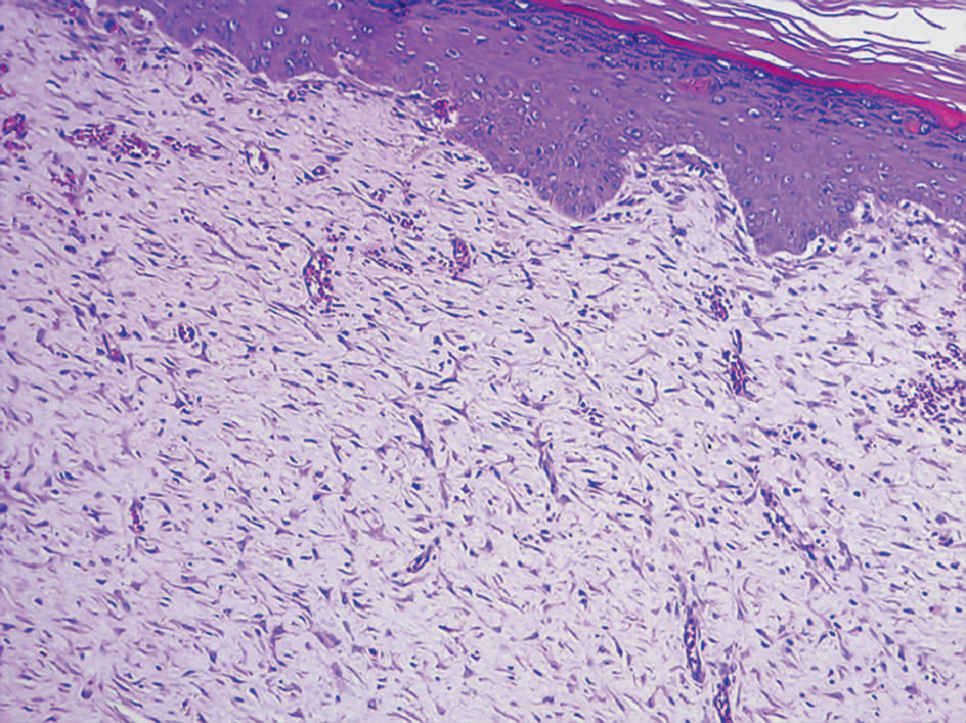
\includegraphics{./images/Image00028.jpg}
	\caption{肉芽组织转变为瘢痕组织镜下观(HE染色,低倍) \\ {\small 毛细血管明显减少,胶原纤维沉积增多}}
	\label{fig2-5}
\end{figure}

瘢痕组织中血管少,细胞少,胶原纤维较多较粗,常有玻璃样变性。由于瘢痕组织内肌纤维母细胞的收缩及后期瘢痕内水分明显减少,引起病灶体积缩小,此即瘢痕收缩。瘢痕收缩可引起组织、器官表面凹陷或器官变形,还可造成腔道狭窄。关节附近的瘢痕可致关节运动障碍。瘢痕愈大,影响愈甚。发生在重要器官的瘢痕收缩后将造成严重后果。例如,心瓣膜上的瘢痕可引起瓣膜闭锁不全或瓣膜口狭窄,造成血流动力学的改变,严重者可导致心力衰竭。一般情况下,瘢痕中的胶原纤维在胶原酶的作用下逐渐降解吸收,瘢痕缓慢变小、变软,偶尔瘢痕中胶原纤维形成过多,可成为大而不规则的硬结。少数“瘢痕体质”者,轻微创伤后就可形成明显的瘢痕,过度的瘢痕形成称为瘢痕疙瘩。

\section{创伤愈合}

创伤愈合(wound
healing)是机体组织遭受创伤后进行再生修复的过程,它包括创伤周围特异性组织细胞再生,以及肉芽组织形成、纤维化,最后形成瘢痕组织的复杂过程。

\subsection{创伤愈合的基本过程}

\paragraph{伤口的早期变化}
伤口局部有不同程度的组织损伤、出血及炎症反应。血液和炎性渗出物中的纤维蛋白凝固成血凝块充满缺口,血凝块表面脱水、干燥形成痂皮。血凝块和痂皮对伤口起填充和保护作用,血凝块中的血小板及单核细胞等具有促进局部细胞再生的作用。

\paragraph{伤口收缩}
2~3天后,伤口边缘的皮肤和皮下组织向中心移动,创面缩小。动物实验证明,有些部位的创面在15天内可缩小80%,对愈合十分有利。创面缩小与肉芽组织中肌纤维母细胞收缩有关。

\paragraph{肉芽组织增生及瘢痕形成}
大约从第3天开始,自创缘长出肉芽组织,并向伤口中的血凝块内延伸,机化血凝块。第5~6天起,纤维母细胞产生胶原纤维,其后一周胶原纤维形成极为活跃,以后逐渐缓慢下来。随胶原纤维增多,形成瘢痕组织,大约在伤后一个月瘢痕完全形成。瘢痕组织抗拉力的强度只有正常皮肤的70%~80%,因此腹壁和心脏等部位的较大瘢痕,在内压的作用下可膨出形成腹壁疝或室壁瘤。

\paragraph{表皮及其他组织再生}
表皮再生经过细胞移动、细胞增生及细胞分化三个连续过程。受伤后24小时内,创缘上皮基底层细胞,开始在血凝块下面向伤口中心移动、增生,伤后48小时连接成片,形成菲薄的单层上皮,然后分化。伤后5天内就可恢复原有上皮层厚度并具有角化层的正常表皮结构。

如伤口过大(直径>20
cm)再生表皮难以将创口完全覆盖,往往需要植皮。毛囊、汗腺、皮脂腺等组织若完全破坏,则不能再生,由瘢痕修复。

\subsection{皮肤的创伤愈合}

根据创伤程度及有无感染可分为三种类型。

\paragraph{一期愈合(healing by first intention)}
见于组织缺损少、创缘整齐、创面对合好、无感染、炎症反应轻微的伤口。例如手术切口,切口内只有少量血凝块,创缘炎症反应轻微,第二天表皮再生,在48小时内形成连续的上皮细胞层,覆盖创面,将之与炎性渗出物及血凝块分开。第三天肉芽组织从创缘长出并很快填满伤口,5~6天胶原形成(此时可拆线),2~3周完全愈合,留下一条线状瘢痕(图\ref{fig2-6})。

\begin{figure}[!htbp]
	\centering
	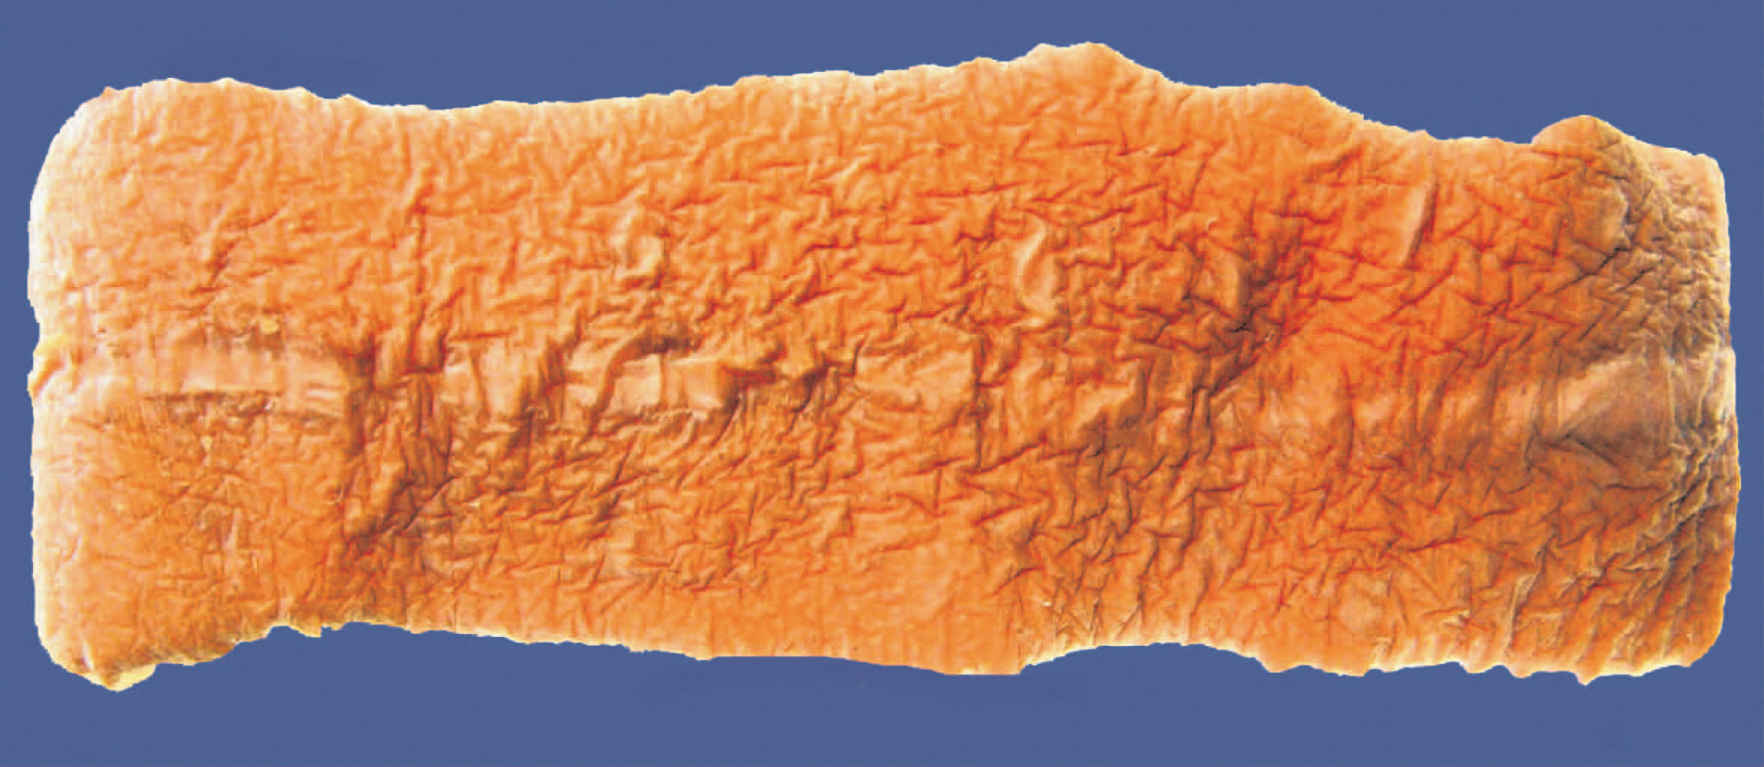
\includegraphics{./images/Image00029.jpg}
	\caption{皮肤一期愈合}
	\label{fig2-6}
\end{figure}

\paragraph{二期愈合(healing by second intention)}
见于创伤组织缺损大,创缘不整齐,伴有感染,炎症反应明显的伤口。愈合由创伤底部向上进行,由于创伤大,需要较多的肉芽组织才能填补缺损,这类创伤坏死组织出血多,并有感染,影响上皮细胞增生移行及肉芽组织的生长,需要清除坏死组织,控制感染,创伤才能愈合。二期愈合和一期愈合的基本过程相同,但需时较长。由于二期愈合肉芽组织增生明显,愈合后形成的瘢痕较大(图\ref{fig2-7}),常影响脏器的外形和功能。若条件允许,可行清创术以达到一期愈合的目的。

\paragraph{痂下愈合(healing under scar)}
创伤表面的血液、渗出液及坏死组织凝固干燥,形成黑褐色硬痂,在痂下进行上述的愈合过程(图\ref{fig2-8}),待上皮再生完成后,硬痂脱落。其愈合时间通常较无痂者长。如痂下有较多的渗出液,易继发感染,不利于愈合。
\begin{figure}[!htbp]
	\centering
	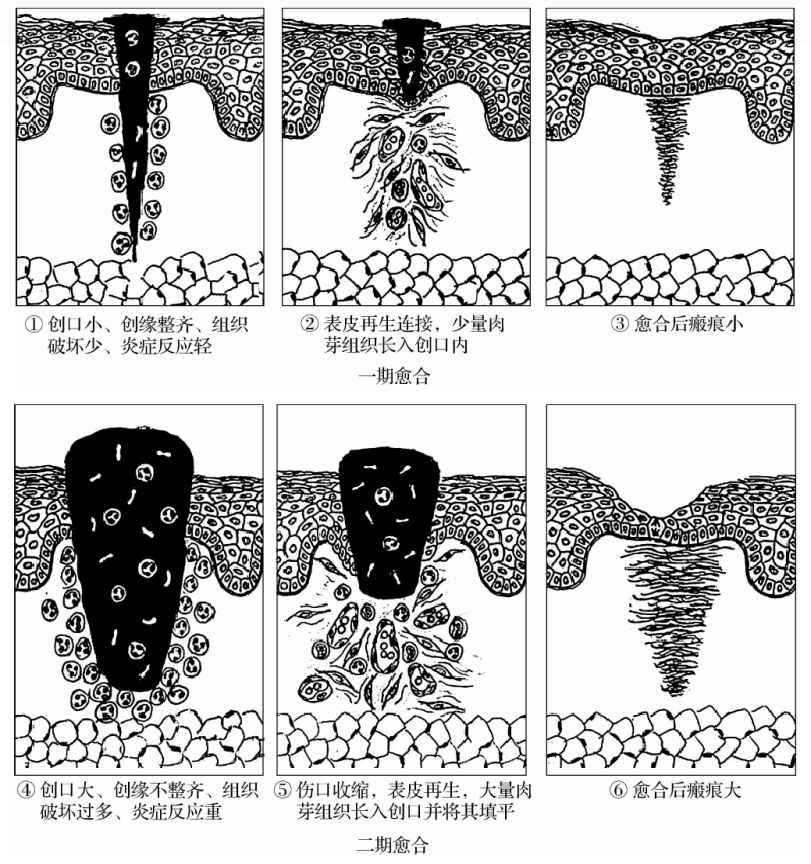
\includegraphics{./images/Image00030.jpg}
	\caption{创伤愈合}
	\label{fig2-7}
\end{figure}

\begin{figure}[!htbp]
	\centering
	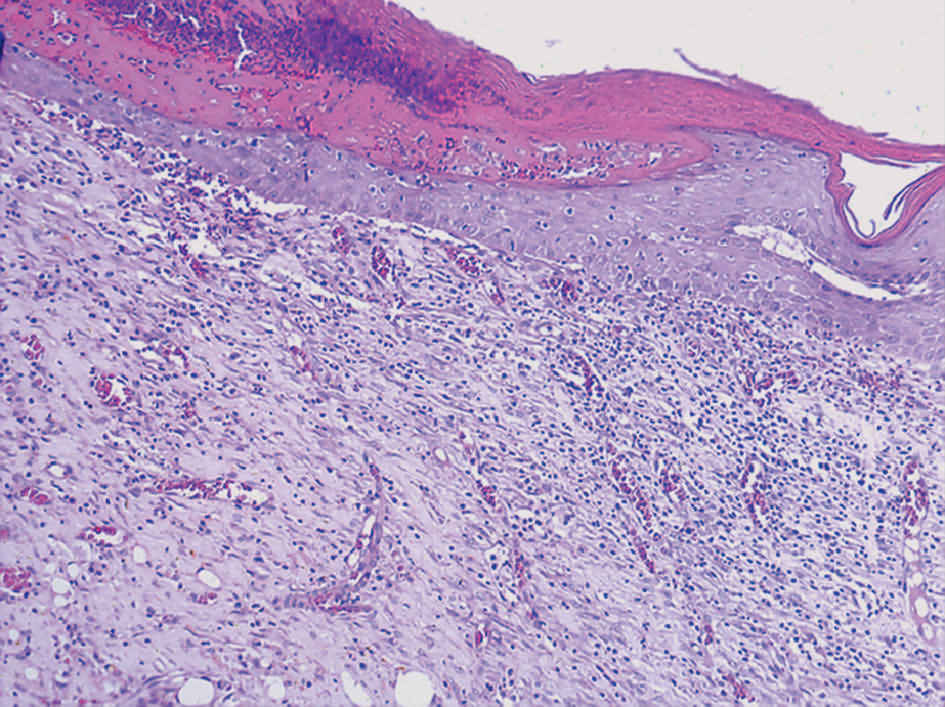
\includegraphics{./images/Image00031.jpg}
	\caption{痂下愈合(HE染色,低倍){\small 皮肤创面有血痂形成,上皮已经再生完成,肉芽组织内仍有较多的炎细胞浸润}}
	\label{fig2-8}
\end{figure}


\subsection{骨折愈合}

骨折通常可分为外伤性骨折和病理性骨折两大类。骨的再生能力很强,骨折后大都能完全恢复,其愈合基础是骨膜细胞再生。因其结构和功能的特殊性,愈合过程较复杂,可分为以下几个阶段(图\ref{fig2-9})。

\begin{figure}[!htbp]
	\centering
	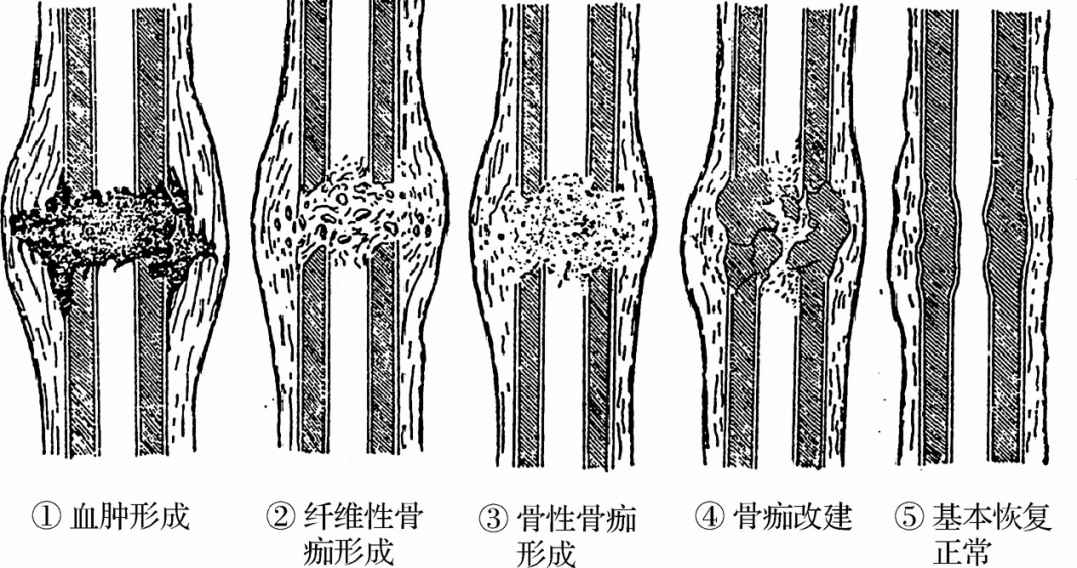
\includegraphics{./images/Image00032.jpg}
	\caption{骨折愈合过程}
	\label{fig2-9}
\end{figure}

\paragraph{血肿形成}
骨折时,局部骨和软组织受损伤,血管破裂出血,填充在骨折两端及其周围组织间,形成血肿。骨折局部还可见轻度的炎症反应。

\paragraph{纤维性骨痂形成}
骨折2~3天后,血肿开始由肉芽组织取代而机化,增生的肉芽组织填充和桥接骨折断端,使局部呈梭形膨大,继而纤维化,称为纤维性骨痂,起到初步固定作用。

\paragraph{骨性骨痂形成}
骨折愈合过程进一步发展,纤维性骨痂逐渐分化出骨母细胞及软骨母细胞。骨母细胞分泌基质,逐渐成熟为骨细胞,形成类骨组织,类骨组织经钙盐沉着后变为骨组织,即骨性骨痂。此过程约需几周。骨性骨痂中骨小梁排列紊乱,结构不够致密,仍达不到正常功能需要。软骨母细胞也可经过软骨内化骨形成骨性骨痂,但所需时间较长。软骨的形成与骨折后断端固定不良有关。

\paragraph{骨痂改建或再塑}
上述骨痂形成后,骨折断端被幼稚的、排列不规则的编织骨连接起来,属临床愈合。为了适应生理要求,还需要进一步改建为成熟的板状骨,并重新恢复皮质骨和骨髓腔的正常关系。改建是在破骨细胞的骨质吸收及骨母细胞新骨形成协调作用下进行的。改建后新骨的排列将适应该骨活动时承受压力的方向。骨痂的改建过程在儿童需1~2年,成人需要更长时间。

\subsection{影响创伤愈合的因素}

影响创伤愈合的因素多种多样,了解的目的是为了避免不利因素,创造有利条件,加速组织再生修复。

\subsubsection{全身因素}

\paragraph{年龄}
儿童和青少年较老年人组织再生能力强,愈合快。这可能与老年人常有动脉粥样硬化、血液供应减少、代谢减慢、免疫力降低等有关。

\paragraph{营养}
营养物质缺乏,特别是蛋白质和维生素C,对愈合有很大影响。长期蛋白质缺乏,其中含硫氨基酸蛋氨酸、胱氨酸缺乏时影响前胶原分子形成,不仅使创面愈合速度减慢,而且抗张力强度减低。锌缺乏时将影响DNA和RNA的合成,细胞增生缓慢,延缓创伤愈合。

\paragraph{疾病}
某些疾病,如糖尿病、尿毒症、肿瘤恶病质及一些免疫缺陷病等均可影响再生修复。糖尿病患者白细胞功能降低,对细菌微生物的易感性增加。此外,凡引起小血管闭塞及神经的病变都将影响愈合。

\paragraph{激素}
特别是皮质醇类激素能抑制炎症的渗出反应。临床上用皮质醇处理的病人,创伤处巨噬细胞稀少,影响肉芽组织的形成和创伤收缩。因此,在炎症修复过程中皮质醇类激素的使用要慎重。

\subsubsection{局部因素}

\paragraph{感染和异物}
感染使渗出物增多,从而增加局部创口的张力,甚至引起伤口裂开。许多化脓菌产生的毒素和酶能引起组织坏死,基质和胶原纤维溶解,加重局部损伤,因此只有当创伤局部感染被控制后,修复才能顺利进行。异物(如丝线等)可对局部组织有刺激作用,引起异物反应,妨碍修复。

\paragraph{局部血循环障碍}
血液供应对创伤愈合很重要,凡是引起动脉血供应不足,或静脉血流不畅的疾病都将影响局部创伤的愈合。如下肢静脉曲张患者,小腿发生溃疡后,常迁延不愈,变为慢性溃疡。X线长期照射的部位,小动脉壁增厚,管腔变窄,局部组织供血不良,损伤后修复缓慢。

\paragraph{神经支配}
正常的神经支配对维持组织结构及功能极为重要,失去神经支配的组织就失去了对损伤的反应。正常的神经功能与再生修复亦有一定关系,例如麻风病引起的溃疡不易愈合,这与麻风病患者肢体神经受累有关。

\section{再生修复的机制}

组织损伤修复的机制极为复杂,涉及损伤局部的炎症反应、各种化学因子的释放、干细胞和纤维母细胞的激活和增殖、细胞外基质的产生以及与细胞之间的相互作用、增生程度的控制、修复后重塑等(图\ref{fig2-10})。

\begin{figure}[!htbp]
	\centering
	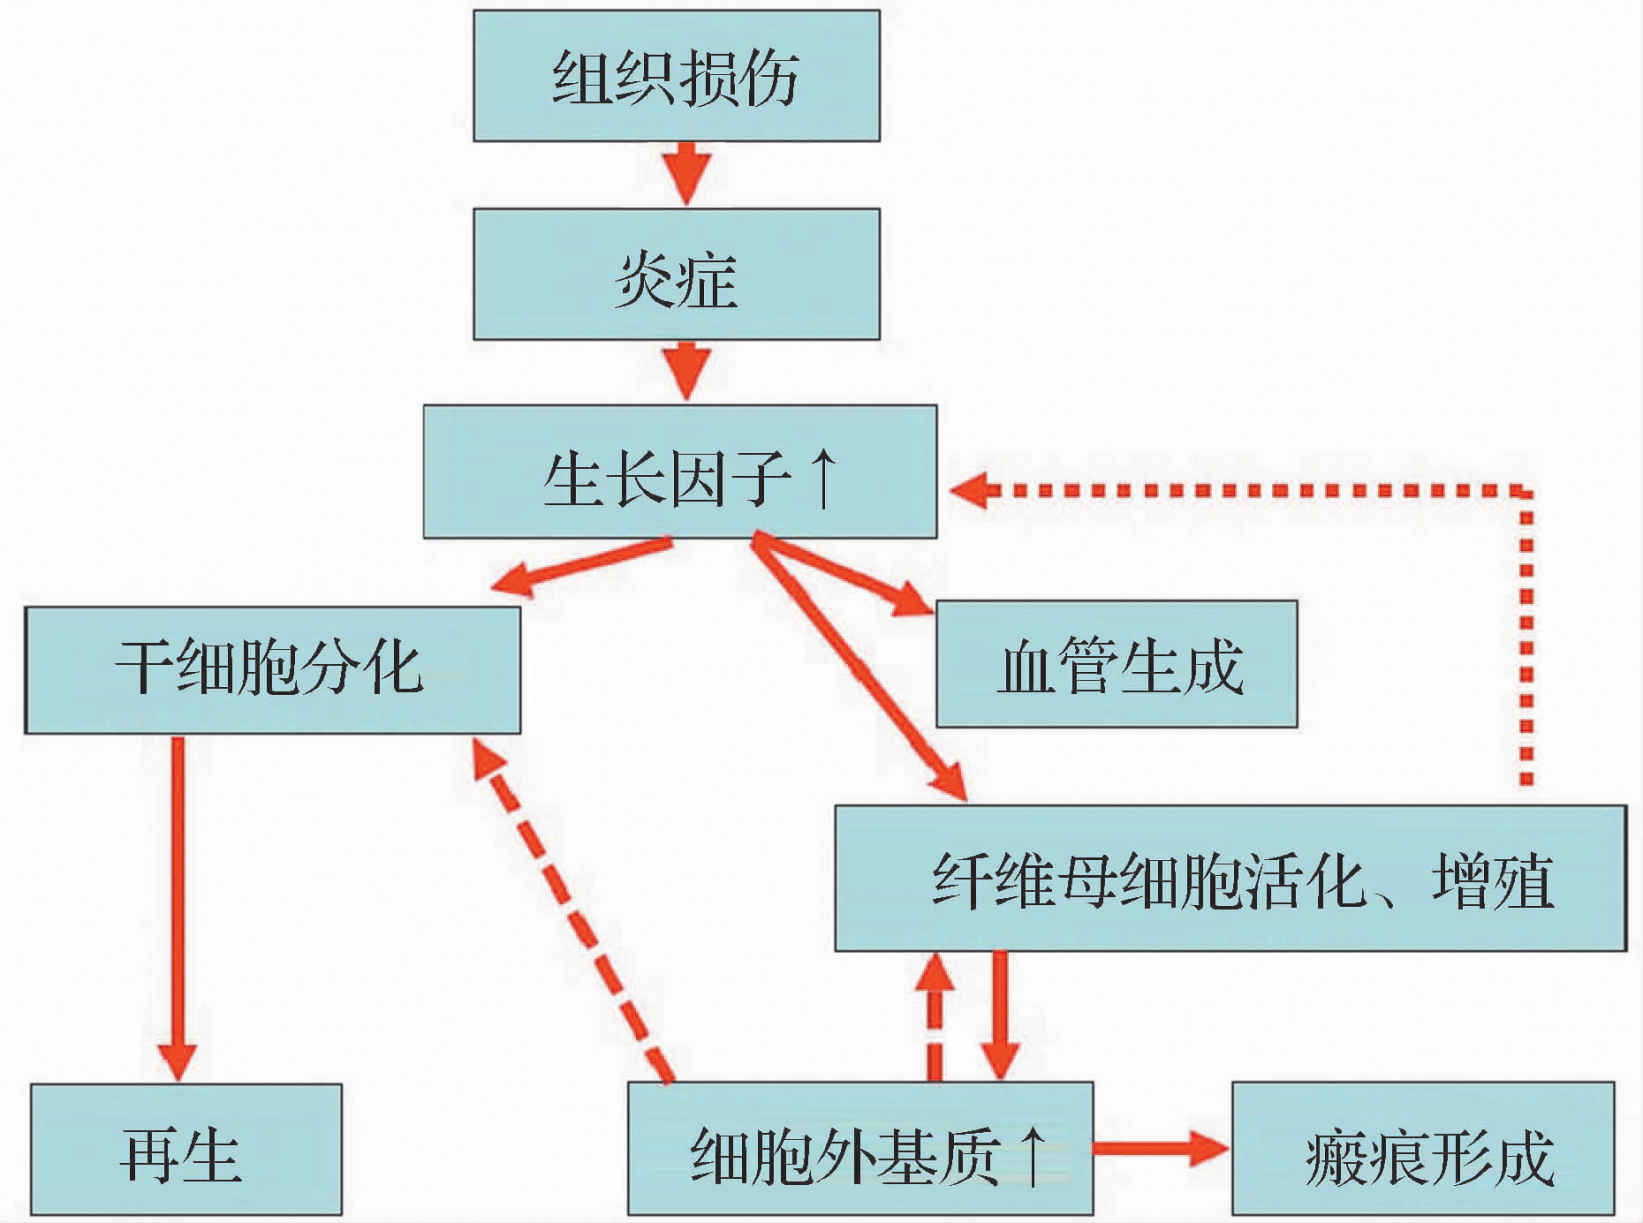
\includegraphics{./images/Image00033.jpg}
	\caption{损伤修复机制}
	\label{fig2-10}
\end{figure}


\subsubsection{干细胞}

干细胞(stem
cell)是一类未充分分化且具有自我复制能力(self-renewing)的多潜能细胞。在一定条件下,它可以分化成多种功能细胞。根据干细胞所处的发育阶段分为胚胎干细胞(embryonic
stem cell,ES细胞)和成体干细胞(somatic stem
cell),近年科学家还在实验室用基因工程方法构建了诱导型多能干细胞。根据干细胞的发育潜能分为三类:全能干细胞(totipotent
stem cell,TSC)、多能干细胞(pluripotent stem
cell)和单能干细胞(unipotent stem
cell)(专能干细胞)。干细胞具有再生各种组织器官和人体的潜在功能。

组织损伤后,干细胞激活,可向特定方向分化、增殖,修复组织缺损。

\subsubsection{生长因子}

细胞受到损伤因素刺激后,可通过释放多种生长因子(growth
factor),刺激同类细胞或同一胚层发育来的细胞增生,促进修复过程。生长因子在细胞移动、收缩和分化中也发挥重要作用。常见的有以下几种:

\paragraph{血管内皮生长因子(vascular endothelial growth factor,VEGF)}
是至今发现的最强的血管通透促进剂,可促进内皮细胞增殖,在胚胎发育、创伤愈合等生理及病理过程中具有明显的促血管增生作用。

\paragraph{纤维母细胞生长因子(fibroblast growth factor,FGF)}
具有广泛的生物学活性,能影响多种细胞(血管内皮细胞、平滑肌细胞、纤维母细胞等)的生长、分化及功能。FGF可使血管内皮细胞分裂并诱导其产生蛋白溶解酶,后者溶解基膜,便于内皮细胞穿越生芽。

\paragraph{血小板源性生长因子(platelet derived growth factor,PDGF)}
主要由黏附于血管损伤处血小板的α颗粒释放,能刺激血管平滑肌细胞、纤维母细胞和胶质细胞等的分裂、增殖,通过刺激胶原合成和胶原酶的活化作用,调节细胞外基质的更新。

\paragraph{表皮生长因子(epidermal growth factor,EGF)}
通过作用于靶细胞膜上的特异性受体而发挥多种生物学效应,是一种强有力的促细胞分裂、分化和增殖的因子,对上皮细胞、纤维母细胞、平滑肌细胞都有促进增殖的作用。

\paragraph{转化生长因子(transforming growth factor,TGF)}
TGF-α可与EGF受体结合,与EGF具有类似作用。TGF-β具有复杂的生物学功能,对纤维母细胞和平滑肌细胞增生的作用依其浓度而异,高浓度可抑制
PDGF受体表达,使其生长受到抑制,低浓度诱导PDGF合成、分泌。

\paragraph{肿瘤坏死因子(tumor necrosis factor,TNF)}
是多功能的多肽,可促进内皮细胞分化,诱导基质产生,也可间接刺激其他细胞产生血管生长因子。在体内可促进内皮细胞形成血管,在体外可刺激培养的内皮细胞形成管样结构。

\subsubsection{细胞外基质及其受体}

人体各种组织均由细胞外基质(extracellular
matrix,ECM)构成支架,它的主要作用是把细胞连接在一起,借以支撑和维持组织的生理结构和功能。ECM能影响细胞的形态、分化、迁移、增殖和生物学功能,在调控胚胎发育、创伤修复及肿瘤浸润转移等方面都起着重要作用。研究表明,尽管不稳定细胞和稳定细胞都具有完全再生能力,但能否重新构建为正常结构尚依赖ECM。

ECM的主要成分如下:

\paragraph{胶原蛋白和弹力蛋白}
胶原蛋白(collagen)是ECM的主要组成成分,几乎分布于所有组织中,为多细胞生物提供细胞外支架。目前发现的胶原类型达18种之多,其中Ⅰ~Ⅳ型含量较多。Ⅰ、Ⅱ、Ⅲ型胶原为纤维性胶原,Ⅰ和Ⅲ型主要分布于间质结缔组织中,Ⅱ型胶原则主要分布于软骨;Ⅳ型胶原为基底膜胶原,在基底膜主要基质蛋白成分中占60%。弹力蛋白(elastin)分子结构与胶原蛋白相似,但分子间交联较少。主要存在于血管、皮肤、韧带、肺等组织中,分子量约70kD,对维持组织的弹性与张力起重要作用。

\paragraph{蛋白多糖}
蛋白多糖(proteoglycans)是ECM的另一重要成分,其结构包括核心蛋白及与其相连接的多糖或多个多糖聚合形成的氨基多糖(glycosaminoglycans)。常见的蛋白多糖有硫酸肝素、硫酸软骨素、硫酸皮肤素、硫酸角质素和透明质酸等,其功能主要是通过介导一系列生物大分子之间的信息传递参与组织的发育和维持正常的生理功能。透明质酸是大分子蛋白多糖复合物的骨架,与调节细胞增殖和迁移有关。

\paragraph{黏附性糖蛋白}
黏附性糖蛋白(adhesive
glycoproteins)既能与其他细胞外基质结合,又能与特异性的细胞表面蛋白结合,将不同的细胞外基质与细胞之间联系起来。纤维连接蛋白(fibronectin)作为一种多功能的黏附性糖蛋白,能使细胞与各种基质成分发生粘连,与细胞黏附、细胞迁移等功能直接相关。层黏连蛋白(laminin)可与细胞表面的特异性受体结合,也可与基质成分如IV型胶原和硫酸肝素结合,还可介导细胞与结缔组织基质黏附。

\paragraph{整合素}
整合素(integrins)是位于细胞膜上的细胞外基质受体,对细胞和细胞外基质的黏附起介导作用,可将来自细胞外基质之信号传入细胞。其特殊类型在白细胞黏附过程中还可诱导细胞与细胞间相互作用。

\subsubsection{抑素与接触抑制}

抑素(chalon)具有组织特异性,似乎任何组织都可以产生一种抑素抑制本身的增殖。如已分化的表皮细胞能分泌表皮抑素,抑制基底细胞增殖。当已分化的表皮细胞丧失时,抑素分泌终止,基底细胞分裂增生,直到增生分化的细胞达到足够数量或抑制达到足够浓度为止。TGF-β虽然对某些间叶细胞增殖起促进作用,但对上皮细胞则是一种抑素。此外干扰素-α、前列腺素E2和肝素在组织培养中对成纤维细胞及平滑肌细胞的增生都有抑素样作用。

皮肤创伤,缺损部周围上皮细胞移动,分裂增生,将创伤面覆盖而相互接触时,或部分切除后的肝脏,当肝细胞增生达到原有大小时,细胞停止生长,不至堆积起来。这种现象称为接触抑制(contact
inhibition)。细胞缝隙连接(可能还有桥粒)也许参与接触抑制的调控。

\begin{center}
	\textbf{知识链接}
\end{center}
\chapterabstract{生物敷料可以与伤口密切贴合,保持愈合环境湿润,减轻疼痛,辅助局部使用药物和内源性分子促进伤口愈合。胶原、透明质酸等材料制备的生物敷料不仅具有止血促凝作用,还可影响生长因子(VEGF、FGF、TGF)分泌,诱导多种细胞增殖分化,有利于伤口愈合。}

{【附】与创伤愈合有关的生长因子}

对单核细胞具有趋化作用:PDGF、FGF、TGF-β

纤维母细胞迁移:PDGF、EGF、FGF、TGF-β、TNF

纤维母细胞增殖:PDGF、CTGF、EGF、FGF、TNF

血管生成:VEGF、FGF

胶原合成:TGF-β、PDGF、TNF

分泌胶原酶:PDGF、FGF、EGF、TNF、TGF-β抑制物

\section*{复习与思考}

{一、名词解释}

修复 再生 纤维性修复 稳定性细胞 永久性细胞 肉芽组织 一期愈合

{二、问答题}

1. 试述肉芽组织的结构及其在修复过程中的作用。

2. 影响细胞再生的因素有哪些?

3. 影响创伤愈合的因素有哪些?

4. 试述骨折愈合的基本过程。
